\documentclass[a4paper, 12pt]{article}

\newcommand{\TikZ}{Ti\textit{k}Z}

\usepackage{tikz}

\date{\today}
\title{\TikZ{} Notes}

\author{Brendan Duke}

\begin{document}

\maketitle

\part{Introduction}

\TikZ{} is built on top of two layers: the system layer, and the basic layer.

The system layer provides a generic interface on top of ``drivers'', such as
dvips, which convert DVI files to PDF or postscript files. This is because each
driver has its own syntax.

The basic layer is built on top of the system layer and consists of drawing
commands. The basic layer is minimal in order to ease porting of new graphics
frontends (i.e.\ frontends analogous to \TikZ{} itself). The basic layer
consists of a core, and modules (e.g.\ a shape module).

The \TikZ{} layer uses the basic layer, and provides convenience functions on
top of the basic layer.

\part{Tutorials}

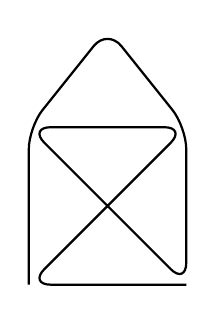
\begin{tikzpicture}
        \draw[thick, rounded corners=8pt]
                (0, 0) -- (0, 2) -- (1, 3.25) -- (2, 2) -- (2, 0) -- (0, 2) --
                (2, 2) -- (0, 0) -- (2, 0);
\end{tikzpicture}

\section{A Picture for Karl's Students}

\end{document}
